\documentclass[11pt]{article}
\usepackage[left=3cm,right=3cm,top=3cm,bottom=3cm]{geometry}
\usepackage{mathptmx}
\usepackage[T1]{fontenc}
\usepackage{titlesec,titling,abstract}
\usepackage{amsmath}
\usepackage{float,graphicx,enumitem}
\usepackage[hidelinks]{hyperref}
\usepackage{../figkit/ixfig}

\titleformat{\section}[block]{\normalfont\fontsize{13pt}{15pt}\bfseries}{\thesection.}{0.5em}{}
\pretitle{\vspace{-6em}\begin{center}\fontsize{14pt}{16pt}\bfseries}
\posttitle{\par\end{center}\vskip 0.5em}
\preauthor{\vspace{0em}\begin{center}\small}
\postauthor{\vspace{-4em}\end{center}}
\renewcommand{\abstractname}{}
\renewcommand{\abstracttextfont}{\normalfont\small}

\begin{document}

\title{Indexus: The Network}
\author{Remi Henriot \\ research@indexus.io}
\date{}
\maketitle

\begin{abstract}
\noindent \textbf{Abstract. }Our whitepaper describes an index in which nodes and data share one binary tree~[2]. This paper describes how a node builds it. A node holds the zones closest to its address, accepts writes for them only when it holds the right to, stores them so that the sum of any zone is read without reading its records, hands zones over without ever letting two nodes write the same one, and sends the sums of its zones to the nodes that hold their parents. We state what is implemented, what was measured, and what is not built yet.
\vspace{1em}\end{abstract}

\section{Introduction}
A node is a program running on one machine with one disk. It has five tasks: hold zones, accept writes, answer sums, move zones when the network changes, and share what it knows with the other nodes. Each task is simple on its own. The difficulty is that nodes learn of each other's changes with some delay, and the protocol must stay correct while they disagree.

We separate what a node \emph{believes} from what it is \emph{allowed} to do. Beliefs, which nodes are active and where data lives, may be late; they only decide where to send a request. Rights, which node may accept writes for a zone, are never inferred from beliefs; they are handed over explicitly and checked on disk.

\section{Nodes}
A node's address is a leaf of the tree: 96 bits, written as a name of 16 characters. A node receives its name when it joins: chosen at random, close to a busy node it is meant to relieve, or so that it takes half of one of the largest parts of the tree.

\begin{figure}[H]
    \centering
    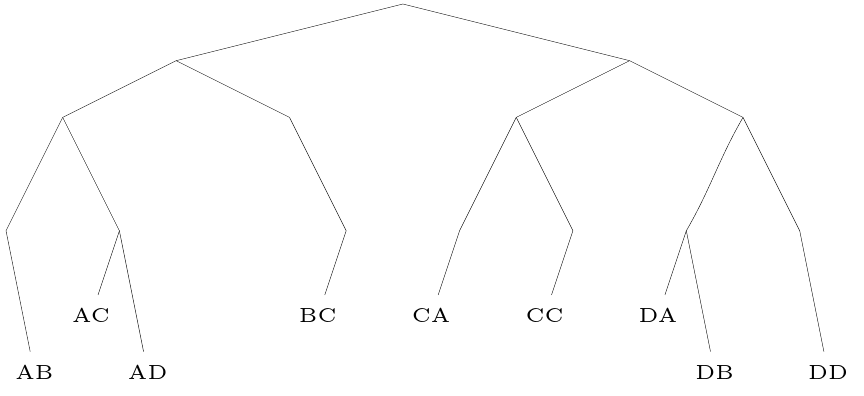
\includegraphics[width=10cm]{orig/network.png}
    \caption{Network of nodes}
\end{figure}

\section{Holding a zone}
A zone's address is its location's bits followed by its collection's name. A zone is held by the active node whose address is closest to it, closeness being the exclusive or of the two addresses read as a number~[3]. The first bit where two addresses differ decides, so the closest node is the one whose path in the tree leaves the zone's path last.

\begin{figure}[H]
    \centering
    \ixnew{figures/owner.tikz}
    \caption{Zone C of collection BB has the address CB. Node CA is the closest: it holds the zone.}
\end{figure}

To find the holder quickly, a node arranges the active addresses in a compressed tree, where each branching tests one bit. Finding the holder of an address follows one branch per test, about $\log_2 N$ tests for $N$ nodes. Two nodes that know the same active nodes always find the same holder.

\section{The right to write}
The holder computed above is a prediction: a node may not know yet that another one has joined. If writes followed that prediction, two nodes could write the same zone while they disagree. The right to accept writes is therefore a separate record.

All rights descend from a first one, covering the whole tree, held by the first node. When a node gives part of its region to another, it writes a certificate that consumes its own right and divides the region into new rights that cover it exactly. A right can be consumed once. For every address there is therefore exactly one current right, and it names one node on one disk.

A node accepts a write only if, inside the transaction that commits it, it finds that the current right for the zone names this node and this disk, that this right is installed on its disk, and that no hand-over of the zone is in progress. A node that only heard of a certificate has not installed it. A late belief can make a write take a longer path, or be refused and retried; it cannot make two nodes accept it.

\section{Writing}
The steps to write a record are:
\begin{enumerate}[leftmargin=1.5em,itemsep=1pt]
  \item The client sends the record and an identifier of its request to any node.
  \item The node tries to commit it. If it does not hold the right, it forwards the record to the node named by the current right, as far as it knows it.
  \item The holder collects the writes that arrive within two milliseconds, up to 256, and commits them together: for each one, the record, the zone's sequence number, a history entry for later hand-overs, and a receipt of the request.
  \item The group is written to disk in one operation. Only then are the records visible to readers, and the holder answers each client.
\end{enumerate}

If a client receives no answer, it sends the same request again. The holder finds the receipt and returns the first answer without writing anything. Receipts are kept for as long as the zone exists and move with it, so a request sent again after a hand-over is still recognised. A write refused in a group does not fail the other writes of the group.

\section{Storage}
A node keeps all its records in one store. A record's key is its collection, its location's bits, the depth of its location and its identifier, in that order. All the records of a zone therefore form one contiguous range of keys, and the ranges of its 64 children follow each other inside it.

\begin{figure}[H]
    \centering
    \ixnew[0.6]{figures/keys.tikz}
    \caption{A zone is one range of keys, and its children are consecutive ranges. Each page stores the sums of its records.}
\end{figure}

The store follows the design of log-structured merge trees~[4]. Writes go to a log on disk and to memory. When memory is full it is written out as a sorted, immutable file, cut in pages of up to 256 records. Each page stores the sums of its records, and each group of 64 pages stores the sums of its pages. Files are merged in the background.

The sum of a zone is read, not maintained. The store adds the sums of the groups and pages that lie entirely inside the zone's range, and reads only the records of the pages at its two edges. The cost depends on the number of pages, not on the number of records. When a record is replaced or deleted, the store writes a second row that carries the previous values negated, so that the sum of all rows always equals the sum of the current records; a merge removes such a row only together with the one it cancels. Sums are kept with a compensation term~[5], so that a negated row cancels its record exactly.

Rights, receipts and sequence numbers are rows of the same store and are committed in the same operations as the records. A crash never separates a record from its receipt or from the right under which it was written.

\section{Moving a zone}
A node that receives too many writes is relieved by a new node whose address differs from its own in a single bit, deeper than any bit it shares with another node. The new node then holds exactly half of the busy node's part of the tree, and no other node loses anything.

\begin{figure}[H]
    \centering
    \ixnew{figures/split.tikz}
    \caption{Node CA is busy. Node CB, one bit away, takes the half of CA's part on its side.}
\end{figure}

The zones of that half move from the old node to the new one. The old node first copies them while it still accepts writes, and sends the writes that arrive meanwhile. Then each zone is handed over in four steps, each written to disk before the next one starts:
\begin{enumerate}[leftmargin=1.5em,itemsep=1pt]
  \item \emph{Freeze.} The old node stops accepting writes for the zone and records its final state.
  \item \emph{Stage.} The new node stores that state and checks its digest.
  \item \emph{Emit.} The old node records that the zone now belongs to the new node. From then on it forwards writes for the zone.
  \item \emph{Install.} The new node installs the zone and the record of the transfer, and accepts writes.
\end{enumerate}

\begin{figure}[H]
    \centering
    \ixnew[0.6]{figures/handoff.tikz}
    \caption{A zone moves. Between freeze and install nobody accepts writes for it; never two nodes.}
\end{figure}

Zones move children first, then parents, up to 64 at a time, so that the other zones of the node keep accepting writes. A step interrupted by a restart is resumed, never undone. When a node has been idle for a while, it hands its whole part to a neighbour whose part contains it, by the same steps, and leaves.

\section{Knowledge}
Each node keeps what it knows of the network: the active nodes, their disks, the rights given and the transfers made. These facts only accumulate, and two nodes that hold the same facts draw the same conclusions, whatever the order in which they learned them.

Facts travel with every message between nodes: a node sends a short digest of what it knows, and the full set only to a node that lacks it. Every ten seconds, a node also contacts one partner in each group of its routing table: the nodes on the other side of the root, those that separate from it one level lower, and so on, rotating among the members of each group.

\begin{figure}[H]
    \centering
    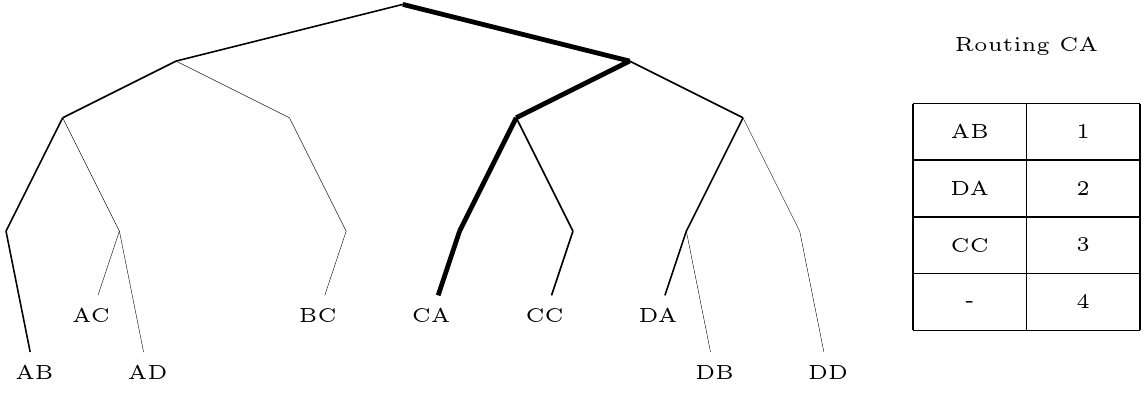
\includegraphics[width=13cm]{orig/routing.png}
    \caption{Routing table (N=4, k=1)}
\end{figure}

Knowledge decides where to send. It never gives a right: learning that a zone was handed over tells a node where to forward writes, not that it may accept them.

\section{Sums across nodes}
A node answers the sums of its zones from its store. When a zone is held by this node and its parent by another, the node is responsible for a \emph{boundary}: it sends the sum of the zone to the holder of the parent.

\begin{figure}[H]
    \centering
    \ixnew{figures/summary.tikz}
    \caption{Zone C, held by CA, sends its sum to zone @, held by BC.}
\end{figure}

The node sends the sum itself, with a version, and never a difference. The parent keeps the latest version received from each child and replaces it; a message received twice or late changes nothing, and a missing message is not counted as zero. The parent's own sum is then its local records, minus its local copies of the remote children, plus their received sums.

After a write, the boundary waits one second and sends the sum as it is then, which covers every write of that second. Sums for the same node are grouped, up to 512 per message. A failed message is retried after 3 seconds, then after longer delays up to 30 seconds. Every five seconds while it is active, and up to every two minutes when it is idle, a node also asks a few other nodes, in rotation, for the sums of its remote children, which repairs any lost message.

\section{Replication}
Today each zone has one copy, on the disk of its holder. A restart loses nothing. A disk lost for good loses the zones it held, and no other node may take them over, since that would give them a second writer.

The design that removes this limit holds each group of zones on three machines. One proposes the writes, and a write is acknowledged once two of the three have stored it. Two majorities of three always share a machine, so the remaining machines hold every acknowledged write, and they choose a new proposer as in Raft~[6]. Rights then belong to the group rather than to one disk. The rules have been checked on a model under randomly injected faults, and the log that counts the majority has been written and tested on its own. Neither is yet used by the running node, and the choice of a new proposer is not written.

\section{Admission}
When a network requires it, a node presents a certificate signed by the network's issuer, and a client presents a token with the scopes it may use, read or write. These credentials decide who may take part. They give no right over any zone. Two limits remain: a node presents its certificate as is, without signing its messages, so its secrecy relies on the encrypted connection; and the issuer does not yet check who asks it for a certificate or a token.

\section{Measurements}
We ran the reference node on rented machines and raised the rate of writes step by step, checking after each step that every acknowledged write could be read back and that every total was exact. From 4 to 16 machines, each node sustained the same rate whatever the size of the network. On 16 machines with local disks, the network acknowledged 52\,440 writes per second. On 32 machines it acknowledged 72\,964 writes per second with no write lost and exact totals, and up to 101\,665 at saturation, 1.94 times the maximum on 16 machines. At that rate the busiest node used most of its processor. Under load, the total of a whole collection included a new write after about one second at the median and four seconds at the 99th percentile.

\section{Calculations}
\textit{Group commit.} With groups of $B$ writes and a disk that takes $f$ to make a group durable, each acknowledged write pays $f / B$ of a disk operation. With $B = 256$, one disk operation serves 256 acknowledgements.

\textit{Hops.} If a client picks its entry node at random among $N$ nodes holding equal parts, a write needs no forward with probability $1/N$ and one forward otherwise.

\textit{Gossip.} A fact reaches every node in at most $d$ rounds, where $d$ is one more than the longest prefix shared by two node addresses, about $2 \log_2 N$ for random addresses. Each node contacts about $\log_2 N + 1$ partners per round. In tests with 1\,024 nodes the bound was 21 rounds and at most 4 were needed.

\textit{Freshness.} A path from a written zone to the root of its collection crosses $k$ boundaries between nodes. With no lost message, the root includes a write after at most $k \times (1\,\mathrm{s} + \text{round trip})$. With balanced addresses, $k$ is 1 up to 64 nodes and 2 up to 4\,096.

\textit{Durability.} If a disk is lost with probability $p$ before it is replaced, a write held on one disk is lost with probability $p$; held on two of three disks, with probability $p^2$. For $p = 0.01$: one in a hundred, against one in ten thousand.

\section{Status}
Implemented and tested: the tree of addresses, holding zones, the rights and their check on disk, writing with receipts, the store and its sums, the hand-over of zones, the relief of busy nodes and the departure of idle ones, knowledge and gossip, and sums across nodes. Measured: the figures of Section~12. Not built: three copies of each zone. Known issue under correction: a write that arrives while its zone's sum is being sent may wait for the next repair round to reach the parent.

\section{Conclusion}
A node holds what is closest to it, writes only what it holds the right to, reads sums from its own storage, and passes zones and sums to other nodes by explicit, durable steps. Beliefs may lag behind the network; rights never do. This is what lets nodes run by different parties share one index without a coordinator, while every acknowledged write is kept once and every total stays exact.

\section*{References}
\begin{enumerate}[label={[\arabic*]},leftmargin=2em,itemsep=1pt]
  \item R. Henriot. Indexus: A Peer-to-Peer Data Indexing System (first version). 2024.
  \item R. Henriot. Indexus: A Peer-to-Peer Data Indexing System. 2026.
  \item P. Maymounkov and D. Mazi\`eres. Kademlia: A Peer-to-peer Information System Based on the XOR Metric. 2002.
  \item P. O'Neil, E. Cheng, D. Gawlick and E. O'Neil. The Log-Structured Merge-Tree (LSM-Tree). 1996.
  \item A. Neumaier. Rundungsfehleranalyse einiger Verfahren zur Summation endlicher Summen. 1974.
  \item D. Ongaro and J. Ousterhout. In Search of an Understandable Consensus Algorithm. 2014.
\end{enumerate}

\end{document}
